\section{Análise preliminar}

Na análise teórica, utiliza-se o software LTspice para realizar a análise numérica do circuito, tanto para os grandes sinais quanto para os pequenos sinais.

\begin{figure}[h]
    \centering
    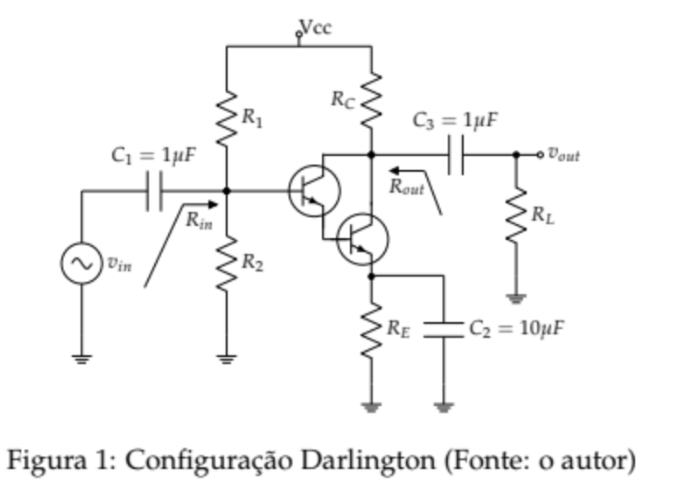
\includegraphics[width=0.5\columnwidth]{Images/o_circuito.png}
    \caption{Circuito em configuração Darlington.}
\end{figure}

\subsection{Análise numérica}

Nesta etapa, monta-se o circuito no LTSpice e verifica-se as tensões e correntes em pontos críticos específicos do circuito. Com esses dados em mãos, é possível calcular as impedâncias e ganhos associados.

\subsection{Circuito no LTSpice}

Simula-se o circuito no LTSpice, utilizando os valores de componentes do projeto, e em modo \emph{DC operating point} que considera os capacitores do circuito como circuitos em aberto.

\begin{figure}[H]
    \centering
    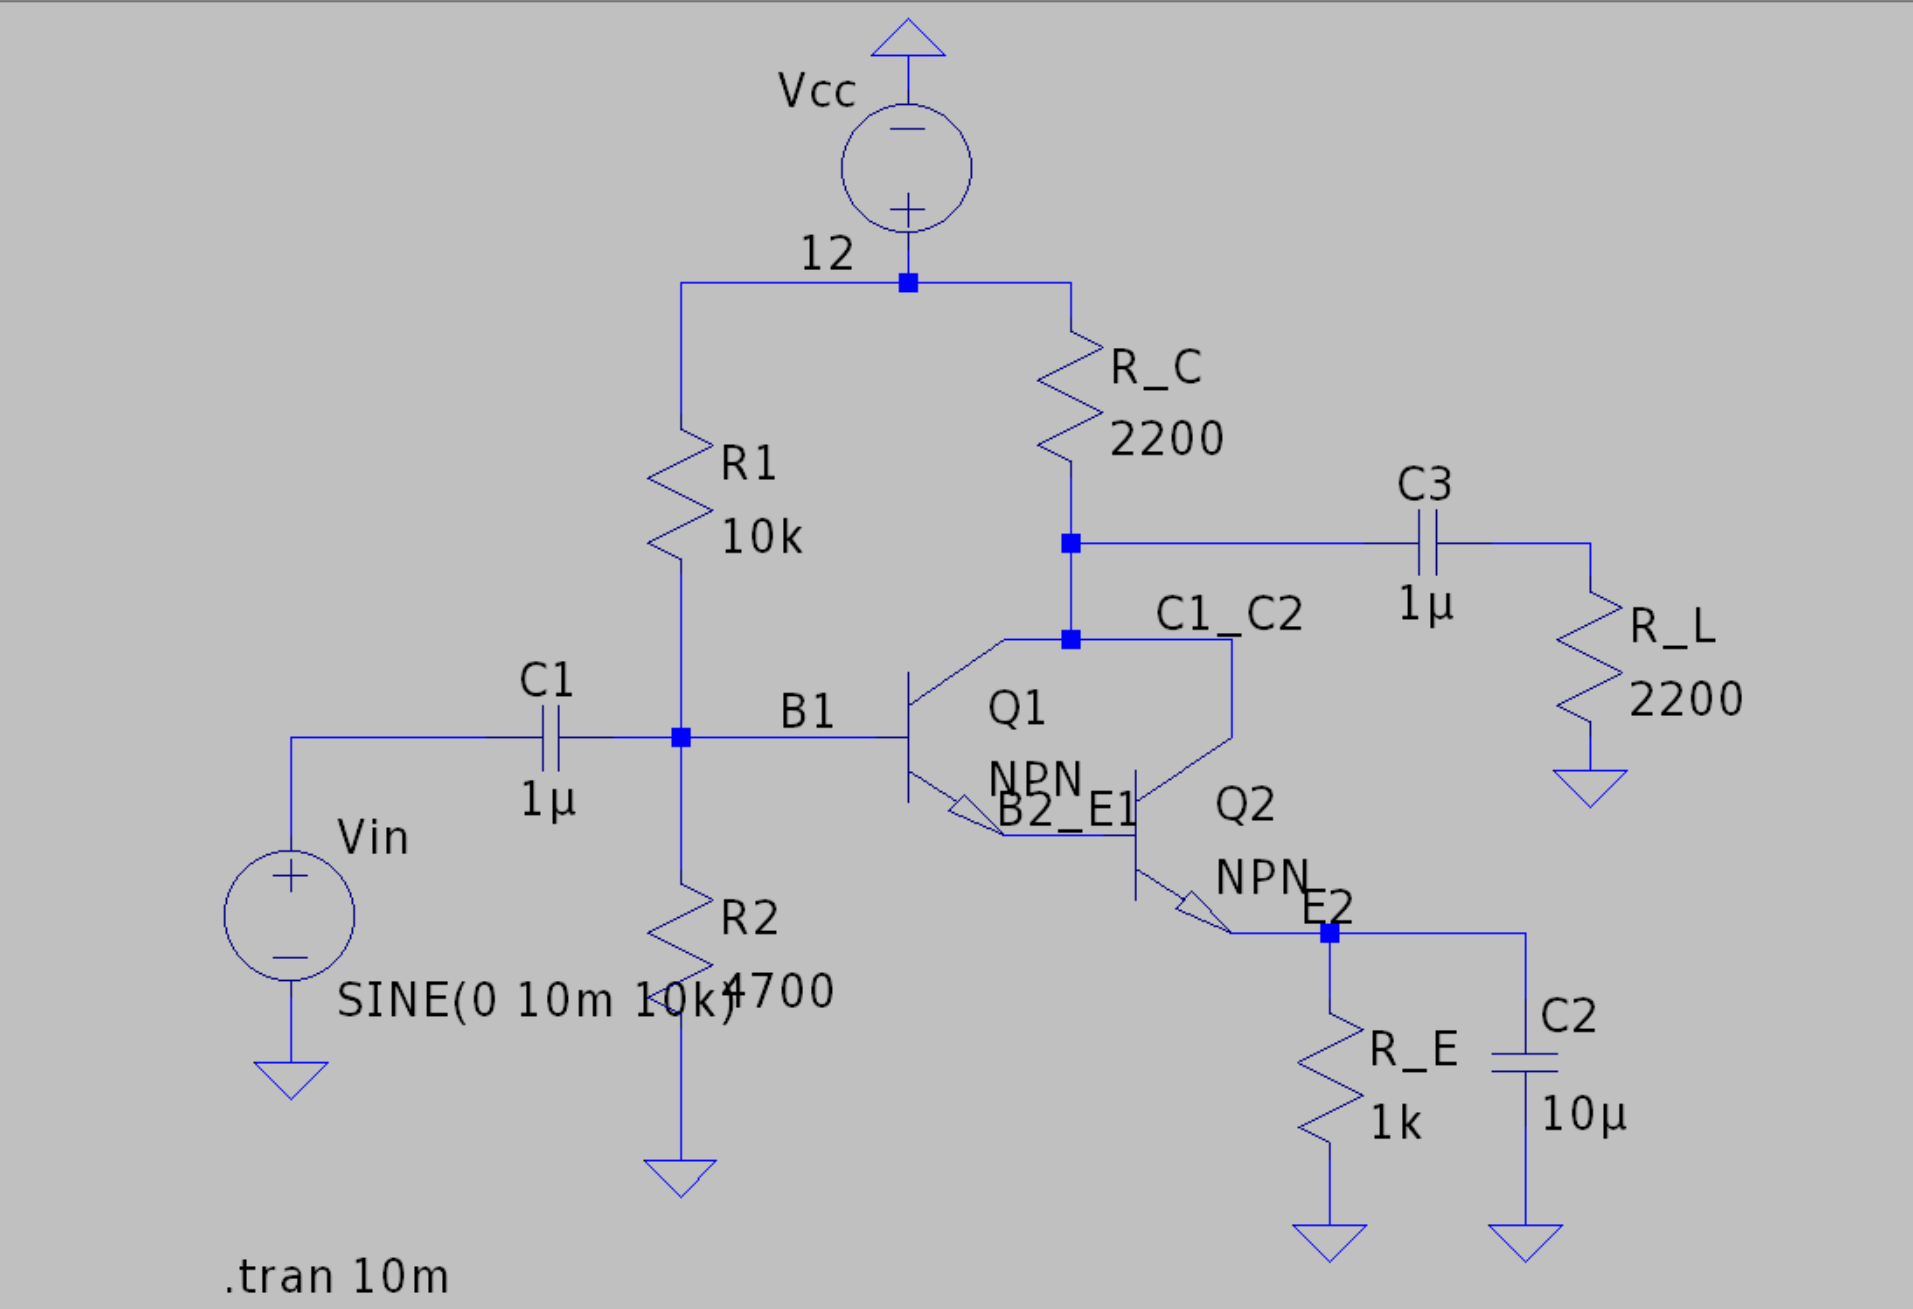
\includegraphics[width=0.5\columnwidth]{Images/o_circuito_ltspice.png}
    \caption{Circuito Darlington simulado no LTSpice.}
\end{figure}

\subsection{Análise de grandes sinais}

Com o circuito simulado com capacitores em aberto podemos obter os valores das tensoes e correntes para grandes sinais. Os valores obtidos estão nas tabelas abaixo.

\subsubsection{Tensão nos transistores}

\begin{center}
    \begin{tabular}{ |c|c| }
        \hline
        Tensão   & Medida    \\
        $V_{C1}$ & $6.80 V$  \\
        $V_{B1}$ & $3.84 V $ \\
        $V_{E1}$ & $3.16 V $ \\
        $V_{C2}$ & $6.80 V$  \\
        $V_{B2}$ & $3.16 V $ \\
        $V_{E2}$ & $2.36 V $ \\
        \hline
    \end{tabular}
\end{center}

\subsubsection{Corrente nos transistores}

\begin{center}
    \begin{tabular}{ |c|c| }
        \hline
        Corrente & Medida        \\
        $I_{C1}$ & $23.2 \mu A$  \\
        $I_{B1}$ & $0.232 \mu A$ \\
        $I_{E1}$ & $23.2 \mu A$  \\
        $I_{C2}$ & $2.36 mA$     \\
        $I_{B2}$ & $23.4 \mu A$  \\
        $I_{E2}$ & $2.36 mA$     \\
        \hline
    \end{tabular}
\end{center}

\subsection{Análise de pequenos sinais}

Com os valores da análise de grandes sinais calculados, podemos realizar a análise de pequenos sinais.

\subsubsection{Calculando parâmetros}

Para obter os ganhos globais e as impedâncias do circuito precisamos obter os parâmetros $g_m$, $r_{\pi}$, e $\beta$ de cada transistor. Para isso, utilizamos as seguintes equações:

\begin{equation}
    \begin{aligned}
        g_m     & = \frac{I_C}{V_T}   \\
        r_{\pi} & = \frac{\beta}{g_m} \\
        \beta   & = \frac{I_C}{I_B}
    \end{aligned}
\end{equation}

E obtemos os seguintes valores:

\begin{center}
    \begin{tabular}{ |c|c| }
        \hline
        Parâmetro   & Valor               \\
        $g_{m1}$    & $9.27 * 10^{-4}$    \\
        $g_{m2}$    & $9.36 * 10^{-2}$    \\
        $\beta_1$   & $100$               \\
        $\beta_2$   & $100$               \\
        $r_{\pi 1}$ & $108 k \varOmega  $ \\
        $r_{\pi 2}$ & $1.07 k \varOmega$  \\
        \hline
    \end{tabular}
\end{center}

\subsubsection{Impedâncias e ganhos}

Com os parâmetros calculados, podemos obter as impedâncias e ganhos do circuito. Para isso, utilizamos as seguintes equações:

\begin{equation}
    \begin{aligned}
        R_{inB_1} & = r_{\pi 1} + (\beta + 1) r_{pi2} \\
        R_{in}    & = R_1 // R_2 // R_{inB_1}         \\
        R_{out}   & = R_C // R_L                      \\
        A_v       & = \frac{-gm R_{out}}{2}
    \end{aligned}
\end{equation}

E obtemos os seguintes valores:

\begin{center}
    \begin{tabular}{ |c|c| }
        \hline
        Parâmetro   & Valor              \\
        $R_{inB_1}$ & $216 k \varOmega$  \\
        $R_{in}$    & $3.15 k \varOmega$ \\
        $R_{out}$   & $1.1k \varOmega$   \\
        $A_v$       & $-51.47$           \\
        \hline
    \end{tabular}
\end{center}
